% Process Hitting

\section{Process Hitting}
\label{sec:ph}

Definition \ref{def:PH} introduces the Process Hitting (PH) framework \cite{PMR10-TCSB}
which allows to model a finite number of local levels,
called \emph{processes},
grouped into a finite set of components, called \emph{sorts}.
A process is noted $a_i$, where $a$ is the sort's name,
and $i$ is the process identifier within sort $a$.
At any time, exactly one process of each sort is \emph{active},
and the set of active processes is called a \emph{state}.

The concurrent interactions between processes are defined by a set of \emph{actions}.
Each action is responsible for the replacement of one process by another of the same sort
conditioned by the presence of at least one other process in the current state.
A normal action is denoted by $\PHfrappe{a_i}{b_j}{b_k}$, which is read as
“$a_i$ \emph{hits} $b_j$ to make it \emph{bounce} to $b_k$”,
where $a_i$, $b_j$, $b_k$ are processes of sorts $a$ and $b$,
called respectively \emph{hitter}, \emph{target} and
\emph{bounce} of the action. 
We also call a \emph{self-hit} any action whose hitter and target sorts are the same,
that is, of the form: $\PHfrappe{a_i}{a_i}{a_k}$. The original Process Hitting framework contains only actions with one hitter but it should be noted that during these last years it was gradually enriched with new type of sorts like cooperative sorts (the same role of a multiplex) and new actions like plural actions \cite{folschette-phd-14} (at least 2 hitters), actions with priority \cite{FPMR13-CS2Bio} and now actions with delays tackled in this paper.

The PH is therefore a restriction of asynchronous automata, where each transition
changes the local state of exactly one automaton,
and is triggered by the local states of at most two distinct automata.
This restriction in the form of the actions was chosen to permit
the development of efficient static analysis methods
based on abstract interpretation \cite{PMR12-MSCS} and recently exhaustive dynamic analysis \cite{benabdallah2015}.

\begin{definition}[Process Hitting]\label{def:PH}
  A \emph{Process Hitting} is a triple $(\PHs,\PHl,\PHa_p)$ where:
  \begin{itemize}
    \item  $\PHs = \{a,b,\dots\}$ is the finite set of \emph{sorts};
    \item  $\PHl = \prod_{a\in\PHs} \PHl_a$ is the set of \emph{states} where
      $\PHl_a = \{a_0,\dots,a_{l_a}\}$
      is the finite set of \emph{processes} of sort $a\in\Sigma$
      and $l_a$ is a positive integer, with $a\neq b\Rightarrow \PHl_a \cap \PHl_b = \emptyset$;
    \item $\PHa_p$ = \{ $\PHfrappe{A}{b_j}{b_k}$ with $A \in \PHl^{\diamond} \wedge b \in \PHs \wedge b_j \neq b_k \wedge$ if $b_j \in A \Rightarrow A=b_j$\} is the finite set of \emph{actions}.
    With $\PHl^{\diamond}$ the set of all the sub-states of $\PHl$.    
      %$\PHa$ = \{ $\PHfrappe{A}{b_j}{b_k}$ with $A \in \PHl^{\diamond} \wedge b \in \PHs \wedge b_j \neq b_k \wedge$ if $b_j \in A \Rightarrow A=b_j$ \}.With $\PHl^{\diamond}$ the set of all the sub-states of $\PHl$. 
  \end{itemize}
\end{definition}

\begin{example}
The figure \ref{fig:ph} represents a $\PH$ $(\PHs,\PHl,\PHa)$ with three sorts
($\PHs = \{a, b, c\}$) and:
$\PHl_a = \{a_0, a_1\}$,
$\PHl_b = \{b_0, b_1\}$,
$\PHl_z = \{z_0, z_1, z_2\}$.
\begin{figure}[ht]
\label{fig:ph} 
\centering
\begin{tikzpicture}[apdotsimple/.style={apdot}]
%\path[use as bounding box] (0,-1) rectangle (4,4);

\TSort{(0,1)}{z}{2}{l}
\TSort{(1.5,4)}{b}{3}{t}
\TSort{(4,1)}{a}{2}{r}

\THit{b_0}{}{z_1}{.east}{z_0}
\THit{a_1}{out=60,in=0,selfhit}{a_1}{.east}{a_0}

\TActionPlur{a_0, b_1}{z_0.north east}{z_1.south east}{}{2,2}{right}

\path[bounce,bend left]
\TBounce{a_1}{}{a_0}{.north}
\TBounce{z_1}{bend left=90}{z_0}{.south east};

\TState{a_1,b_1,z_0}
\end{tikzpicture}
\caption{
A PH model example with three sorts: $a$, $b$ and $z$ ($a$ is either at level 0 or 1, $b$ at either level 0, 1 or 2 and $z$ at either level 0, or 1). Boxes represent the \emph{sorts} (network components), circles represent the \emph{processes} (component levels), and the 3 \emph{actions} that model the dynamics are depicted by pairs of arrows in solid and dotted lines. A self-action:  $\PHfrappe{a_1}{a_1}{a_0}$, a mono-action:  $\PHfrappe{b_0}{z_1}{z_0}$ and a plural action  $\PHfrappe{a_0 \wedge b_1}{z_0}{z_1}$.  The grayed processes stand for the possible initial state: $\PHstate{a_1, b_1, z_0}$.
}
\end{figure}
\end{example}
A state of a given PH consists in a set of active processes containing a single process of each sort.
The active process of a given sort $a \in \PHs$ in a state $s \in \PHl$
is noted $\PHget{s}{a}$.
For any given process $a_i$ we also note: $a_i \in s$ if and only if $\PHget{s}{a} = a_i$. For each sort, it cannot have more than one active process at one state. The dynamics of the PH is performed thanks to the actions. Indeed, the transition from one state $s_1$ to its successor $s_2$ is done when there is a playable action (definition \ref{def:playableAction}) at $s_1$. After each transition only one sort, or one component, changes its level from one process to another.
%
%In some cases it is necessary to represent a reaction of a set of components on one component. For example in the bio-chemical reactions :$X \xrightarrow{Y} Z$ or  $X + Y \rightarrow Y + Z$, where $ X $ is a set of reactives, $ Y $ a set of catalysts and $ Z $ a set of products. % In PH the evolution is asynchronous so we consider that $Z$ is one component. 
%Plural actions permit to represent this kind of reactions in PH. The plural is made up of two sets of processes of different sorts, which represent all the hitters and the bounces. For example the bio-chemical reaction above would be presented in PH by:  $\PHfrappe{X_1 \wedge Y_1}{Z_0}{Z_1}$, if we consider $X$, $Y$ and $Z$ are the sorts, each one is either at level 0 (if it is abscent) or 1 (if it is present).

In some dynamics it is crucial to have information about the delays between two events (two states of a PH). Classic actions, described above, cannot exhibit this information: we just know chronology, i.e., that the state $s_2$ will be after $s_1$ in the next step but it is not possible to know chronometry, i.e., how much time this transition takes to occur. We propose to add the delay in the action attributes which is responsable of the transition between the two states. That means that this timed action (\pref{def:TimedAction}) needs to be played during a specific time so that the system does not change its state until it finishes.

\begin{definition}[Timed action]
\label{def:TimedAction}
Let $\PH = (\PHs,\PHl,\PHa_tp)$ be a timed process hitting and $\PHl^{\diamond}$ be the set of all the sub-states of $\PHl$.
A timed action $h$ of $\PH$ is an action with a delay $D \in \mathds{R}^+$: $$\PHfrappedelay{A}{D}{b_i}{b_j}$$ where $A \in \PHl^{\diamond}$, and $b_i$, $b_j \in \PHl_b$ with  $b_i \not = b_j$ and if $b_i \in A$, $A=b_i$.
\end{definition}
To model biological networks, we used the PH framework with timed actions (\pref{def:PH-timed}). Indeed, in the biological models that we studied we need to present not only the cooperation between the components to influence another one (by \emph{actions}), but also the time needed by this action to make a system change called \emph{delay}. 
\begin{definition}[Process Hitting with Timed Actions]
\label{def:PH-timed}
  A \emph{Process Hitting with timed actions} is a triple $(\PHs,\PHl,\PHap)$ where:
  \begin{itemize}
    \item  $\PHs = \{a,b,\dots\}$ is the finite set of \emph{sorts};
    \item  $\PHl = \prod_{a\in\PHs} \PHl_a$ is the set of \emph{states} where
      $\PHl_a = \{a_0,\dots,a_{l_a}\}$
      is the finite set of \emph{processes} of sort $a\in\Sigma$
      and $l_a$ is a positive integer, with $a\neq b\Rightarrow \PHl_a \cap \PHl_b = \emptyset$;
    \item  $\PHap = \{ \PHfrappedelay{A}{D}{b_j}{b_k}  \mid A \in \PHl^{\diamond}, b_j\neq b_k, b_i \in A \Rightarrow A=b_j\}$
      is the finite set of \emph{timed actions}.
  \end{itemize}
\end{definition}

Duration of actions can now be represented in a Process Hitting model thanks to \emph{timed actions}.
Note that if all actions' delays are set to $0$ it is equivalent to Process Hitting without delays (original PH).
The way these new actions should be used is described as follows.

\begin{definition} [Playable Timed Action]
\label{def:playableAction}
Let $\PH = (\PHs,\PHl,\PHap)$ be a PH with timed actions and $s \in \PHl$ a state of $\PH$.
We say that the timed action $h = \PHfrappedelay{A}{D}{b_i}{b_j}$, with $D \geq 0 $,
is \emph{playable in a state $s$} if and only if
$A \subseteq s$ and $b_i \in s$ (\ie$ \forall a_i \in A, \PHget{s}{a} = a_i$ and $\PHget{s}{b}=b_i$).
\end{definition}

%
The dynamics of the Process Hitting is based on asynchronous evolution (only one action can be played at a time) so we have: $$\PHget{(s \play h)}{b} = b_j \text{ and } \forall c \in \PHs, c \neq b \Rightarrow \PHget{(s \play h)}{c}=\PHget{s}{c}$$
The resulting state of the $\PH$ model ($\PH = (\PHs,\PHl,\PHap)$) after playing a delayed action $h$ at time step $t$ and in a state $s$ is called a \emph{successor} of $s$ and is denoted by $(s \play h)$. This succession of states can be denoted by: $\textsf{state}(\PH, t)=s$ and $\textsf{state}(\PH, t+D)=(s \play h)$ with $delay(h)=D$. The resulting state of a sort $a \in \PHs$ by $\PHget{s}{a}$. 

\begin{definition}[Semantics of Process Hitting with Timed Actions]
\label{def:semantic}
Let $\PH = (\PHs,\PHl,\PHap)$ be a Process Hitting with timed actions. Let $\textsf{state}(\PH, t)=s$ with $s \in \PHl$ and $H_t^s$ be the set of playable timed actions in $s$ at time step $t$. If no action is being played at $t$ and $H_t^s \not = \emptyset$, then exactly one action $h \in H_t^s$ has to be played. Let $D \in \mathds{R}^+$ and $h = \PHfrappedelay{A}{D}{b_i}{b_j}$ and $t_D$ be a time steps such that $t_D - t = D$ so that the semantics of $\PH$ can be expressed as follows:
$$ \forall t' \in [t, t_D [ : \textsf{state}(\PH, t')=s \text{ and } \textsf{state}(\PH, t_D)=(s \play h).  $$
\end{definition}

\begin{figure}
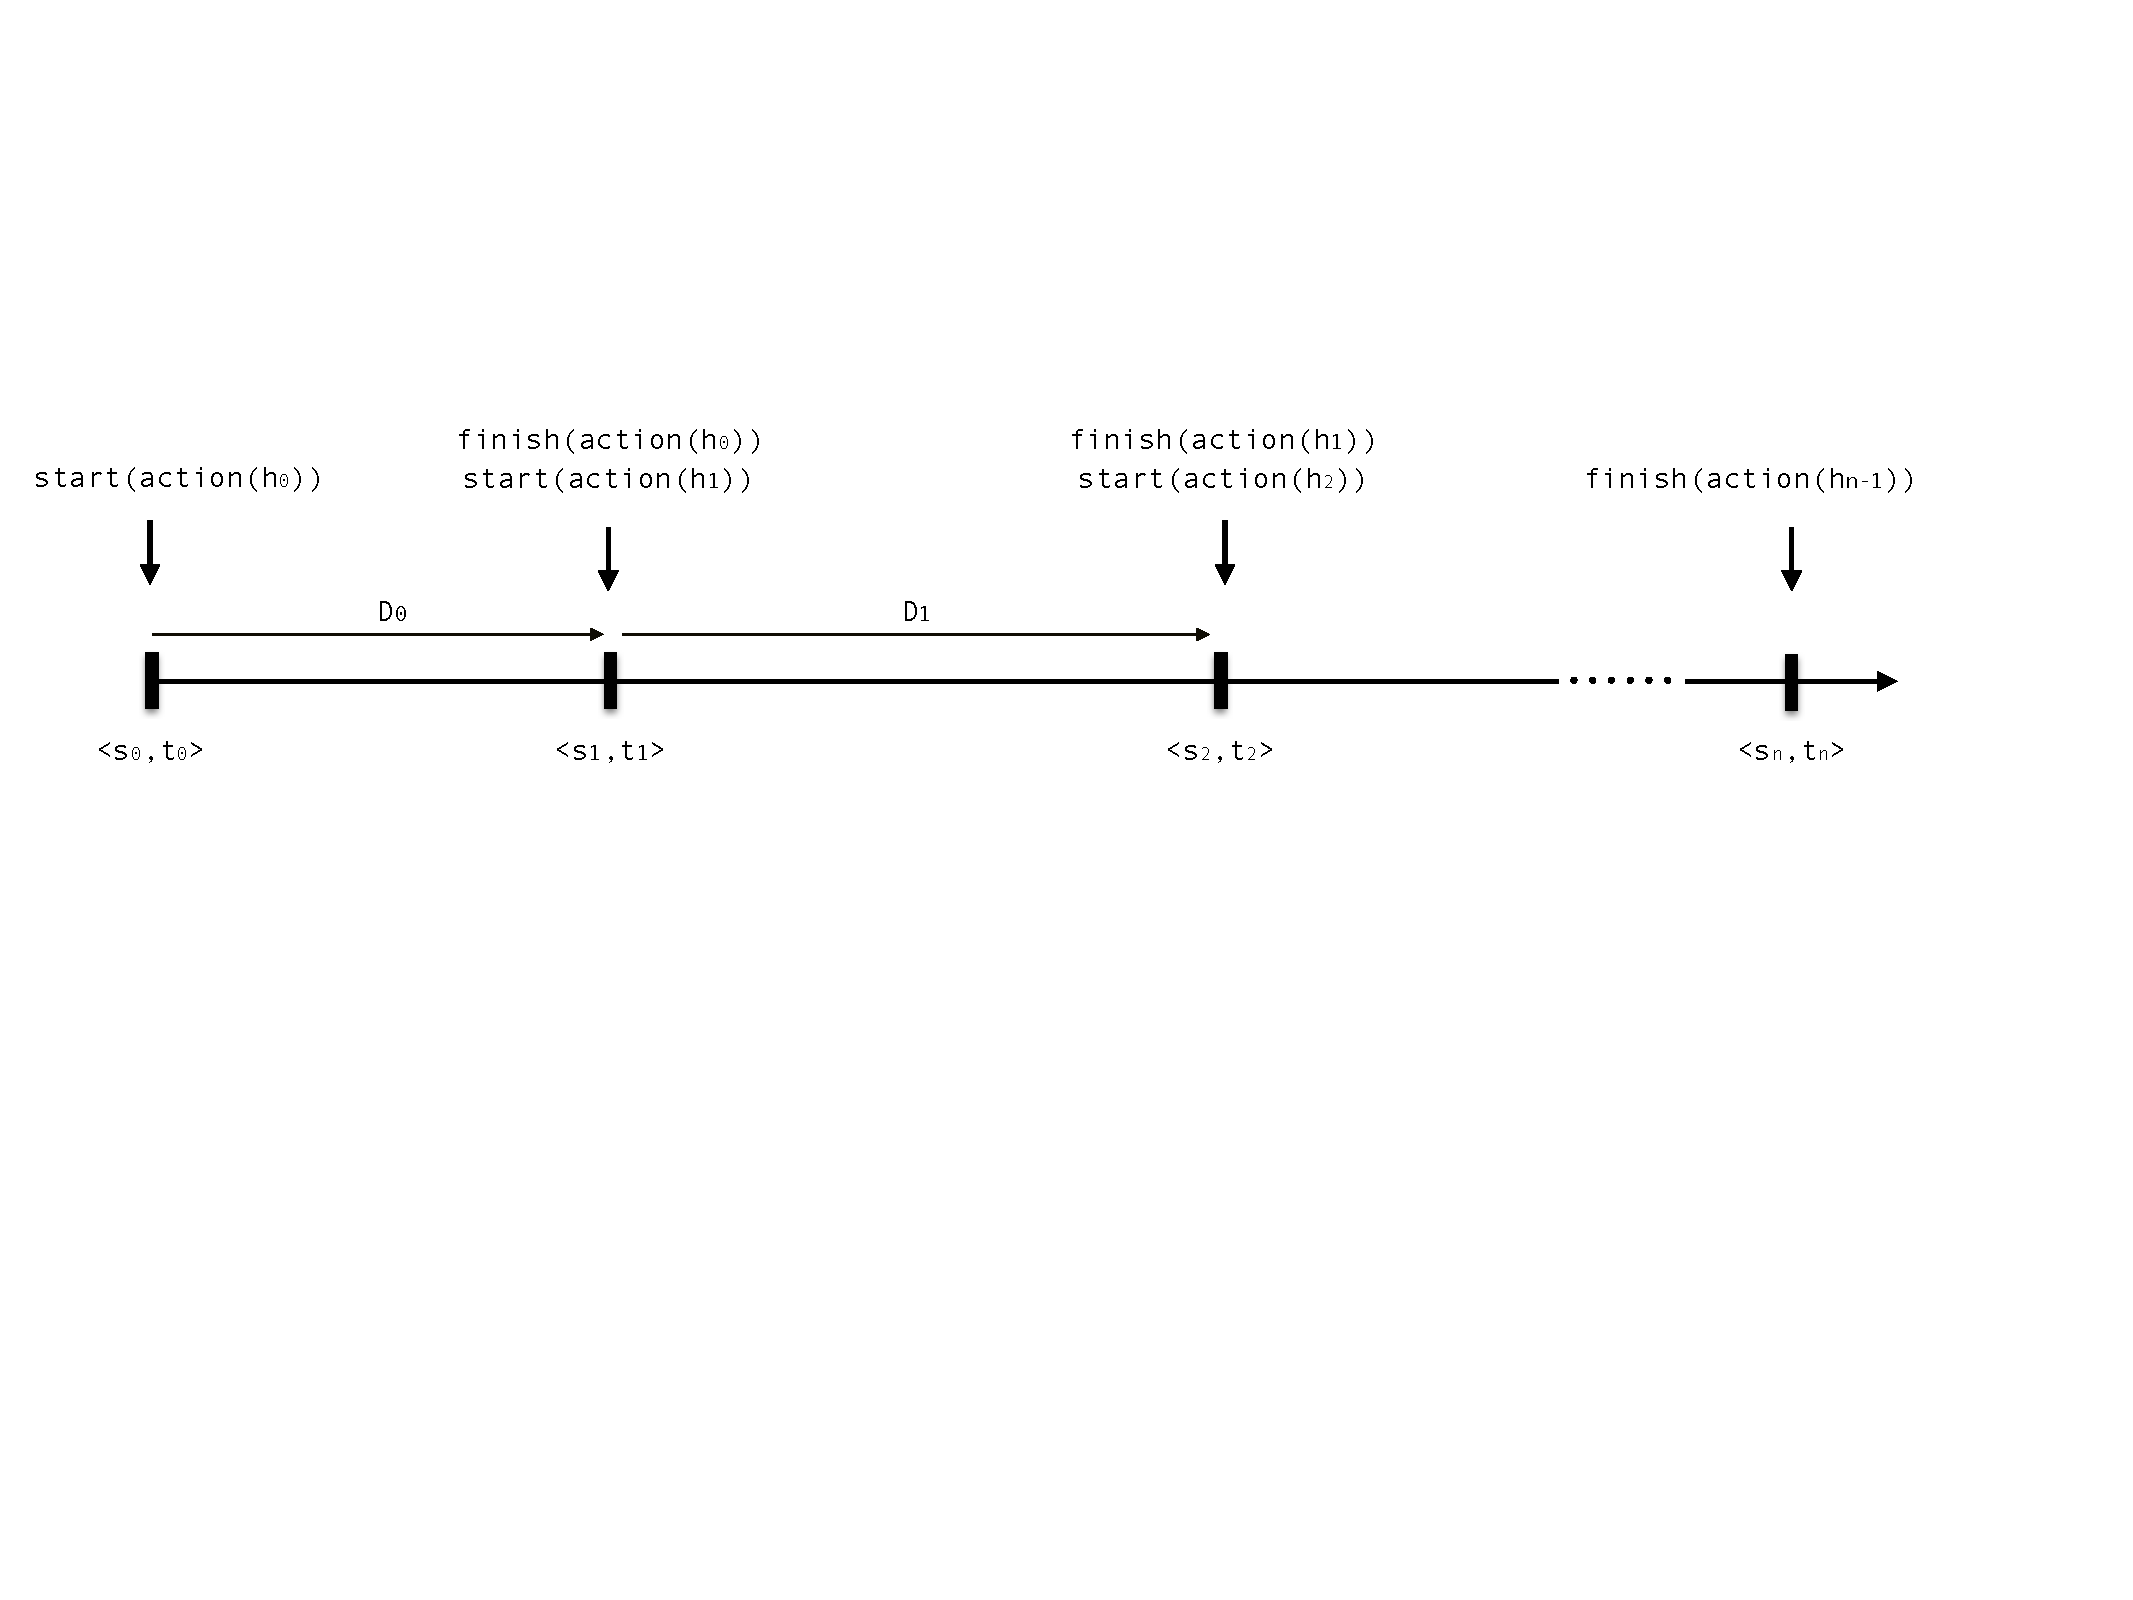
\includegraphics[width=1\linewidth]{images/semantic-timed-PH}
\caption{Semantics of Process Hitting ($\PH = (\PHs,\PHl,\PHap)$) with timed actions such that $\textsf{state}(\PH, t_i)=s_i$, $ \forall t_0 \leq t_i \leq t_n$, and $t_n$ is the maximum time step in the time series data. We mean by $start(action(h_i))$ that the action $h_i$ starts playing so that the system state won't change, from $s_i$ to $s_{i+1}$, until $h_i$ finishestimed actions presented here by $finish(action(h_i))$.}
\end{figure}

%If $\PH = (\PHs,\PHl,\PHap)$ is a dense-time Process Hitting and $s \in \PHl$ be the state of $\PH$ at time $t$ .
We propose in \pref{def:semantic}, the semantics of the timed PH in which we concider to generate the corresponding model to the given observations. Indeed it means that if we consider a PH model $\PH = (\PHs,\PHl,\PHap)$, and if there is no action in $\PHa$ that is playable in $s$, with $s=\textsf{state}(\PH, t)$, the state of the system remains $s$ for all time $t'$ with $t' > t$ (i.e. steady state). If no action are playing (either the initial state or an action just finished) and $h = \PHfrappedelay{A}{D}{b_i}{b_j}$ is the choosen playable action in $s$ then the state of $\PH$ is $s$ during $D$ time steps and at the time step $t+D$
the \emph{successor} of $s$ denoted by $(s \play h)$ is obtained.
\\

Even if there already exists a few hybrid formalisms, we chose to propose this extension of the PH framework. for several reasons.
First, PH is a general framework that,
although it was mainly used for biological networks,
allows to represent any kind of dynamical models,
and converters to several other representations are available.
Indeed, a PH with timed actions is a subclass of temporised petri nets \cite{freedman1991time}.
Although an efficient dynamical analysis already exists for this framework,
based on an approximation of the dynamics,
it is interesting to identify its limits (especially the fact that previous studies were focusing only on discrete, not timed, dynamics)
and compare them to the approach we present later in this paper. Other representations may have required supplementary complexity;
for instance, a labeling would be required
if actions could be triggered by a variable number of processes.
Finally, the particular form of the actions in a  PH model allows
to easily represent them in ASP,
with one fact per action, as described in a previous work \cite{benabdallah2015}. Later we propose the new approch to resolve the generation/revision problem of PH models.

